\chapter{Nonlinear Equations}

One of the most frequently occuring problems in scientific work is to find the roots of
equations of the form 
\begin{align}
    \label{eq:equations form}
    f(x)=0.
\end{align}
In this chapter, we introduce variou iterative methods 
to obtain an approximate solution for the equation (\ref{eq:equations form}).
\par
By approximate solution to (\ref{eq:equations form}) we mean a point $x^*$
for which the function $f(x)$ is very near to zero, ie. $f(x^*)\approx 0$.
\par
In what follows, we always assume that $f(x)$ is continuously differentiable real-valued function 
of a real variable $x$. We further assume that the equation (\ref{eq:equations form}) has only isolated roots,
that is, for each root of (\ref{eq:equations form}) there is a neighbourhood
which does not contain any other roots of the equation.
\par
The key idea in approximating the isolated real roots of (\ref{eq:equations form})
consisting of two steps:
\par
(1) \textbf{Initial guess}: 
Establishing the smallest possible intervals $[a,b]$
constaining one and only one root of the equation (\ref{eq:equations form}).
Take one point $x_0\in [a,b]$ as an approximation to the root of (\ref{eq:equations form}).
\par
(2) \textbf{Improving the value of the root}: If this initial guess $x_0$ is not in desired accuracy, 
then devise a method to improve the accuracy.
\par
\noindent The process of improving the value of the root in step (2) is called the iterative process and
such methods are called iterative methods. A general form of an iterative method may be written as 
\begin{align}
    x_{n+1}=T(x_n),n=0,1,\dots
    \label{eq:iterative method form}
\end{align}
where $T$ is a real-valued function called an iteration function. In the process of iterating a solution,
we obtain a sequence of number $\{x_n\}$ which are expected to converge to the root of (\ref{eq:iterative method form}).

\begin{definition}{Convergence}{Convergence}
    A sequence of iterates $\{x_n\}$ is said to converge with order $p\leqs 1$ to a point $x^*$ if
    \begin{align}
        |x_{n+1}-x^*|\leqs c|x_n-x^*|^p,n\geqs 0
    \end{align}
    for some constant $c>0$.
\end{definition}

\begin{remark}
    If $p=1$, the sequence is said to converge linearly to $x^*$, 
    if $p=2$, the sequence is said to converge quadratically and so on.
\end{remark}

\section{Fixed-Point Iteration Method}
\begin{definition}{}{}
    A fixed point of a function $g(x)$ is a real number $P$ such that $P=g(P)$.
\end{definition}

The key of fixed-point iteration method is to rewrite the equation (\ref{eq:equations form}) in the form
\begin{align}
    \label{eq:fixed point form}
    x=g(x)
\end{align}
so that any solution of (\ref{eq:fixed point iteration form}) ie. any fixed point of $g(x)$ is a solution of (\ref{eq:equations form}).
\begin{example}{}{}
    The equation $x^2-x-2=0$ can be written as\\
    (1) $x=x^2-2$\\
    (2) $x=\sqrt{x+2}$\\
    (3) $x=1+\frac{2}{x}$
\end{example}

For a given nonlinear equation, if it can be written as (\ref{eq:fixed point form}), 
we can set an iterative process of the form (\ref{eq:iterative method form})
with iteration function $g(x)$.
Note that for a given nonlinear equation, this iteration function is not unique.
Once the iteration function is chosen, then the fixed-point iteration method is defined as follows:\\
\textbf{Step 1}: Choose an initial guess $x_0$.\\
\textbf{Step 2}: Define the iteration methods as 
\begin{align}
    x_{n+1}=g(x_n),n=0,1,\dots
    \label{eq:fixed point iterative form}
\end{align}
The crucial point in this method is to choose a good iteration function $g(x)$. 
A good iteration function should satisfy the following properties:\\
(1) For the given starting point $x_0$, the successive approximation $x_n$ given by (\ref{eq:fixed point iterative form}) can be calculated.\\
(2) The sequence $x_1,x_2,...$ converges to some point $\xi$.\\
(3) The limit $\xi$ is a fixed point of $g(x)$, ie., $\xi=g(\xi)$.

The first property is the most needed one as illustrated in the following example.
\begin{example}{}{}
    Consider the equation $x^2-x=0$. We can take $x=\pm \sqrt{x}$ and suppose we define $g(x)=-\sqrt{x}$.
    Since $g(x)$ is defined only for $x>0$, we have to choose $x_0>0$. Thus $x_1=-\sqrt{x_0}<0$ and then $x_2$ cannot be calculated.
\end{example}

Therefore, the choice of $g(x)$ has to be made carefully so that the sequence of iterates can be calculated.
How to choose such a iteration function $g(x)$? 
Since, we expect $x_{n+1}=g(x_n)$, we have to ensure the range of $g(x)$ falls in its domain.
That is,
\par
\textbf{Assumption 1}: $a\leqs g(x)\leqs b$ for all $a\leqs x\leqs b$.
\par 
Let us now discuss about the point $3$. This is a natural expectation since the expression 
$x=g(x)$. To achieve this, we need $g(x)$ to be a continuous function. For if $x_n\rightarrow x^*$ then 
\begin{align*}
    x^*=\lim_{n\rightarrow \infty}x_n=\lim_{n\rightarrow \infty} g(x_{n-1}) = g(\lim_{n\rightarrow \infty} x_{n-1})=g(x^*)
\end{align*}
Therefore, we need 
\par
\textbf{Assumption 2}: The function $g(x)$ is continuous.
\par
Let us now discuss point $2$. This point is well understood geometrically. 
In Fig\ref{img:Fixed-point Iteration Procedure}, 
the figure $(a)$ and $(c)$ illustrated the convergence of the fixed-point iterations 
whereas the figure $(b)$ and $(d)$ illustrated the diverging iterations.
In this geometrical observation, we see that when $g'(x)<1$, 
we have convergence and otherwise, we have divergence. Therefore, we make the assumption.

\textbf{Assumption 3}: The iteration function $g(x)$ is differentiable on $I=[a,b]$.
Futher, there exists a constant $0<K<1$ such that
\begin{align*}
    |g'(x)|\leqs K,x\in I.
\end{align*}

\begin{figure}[htbp]
    \centering
    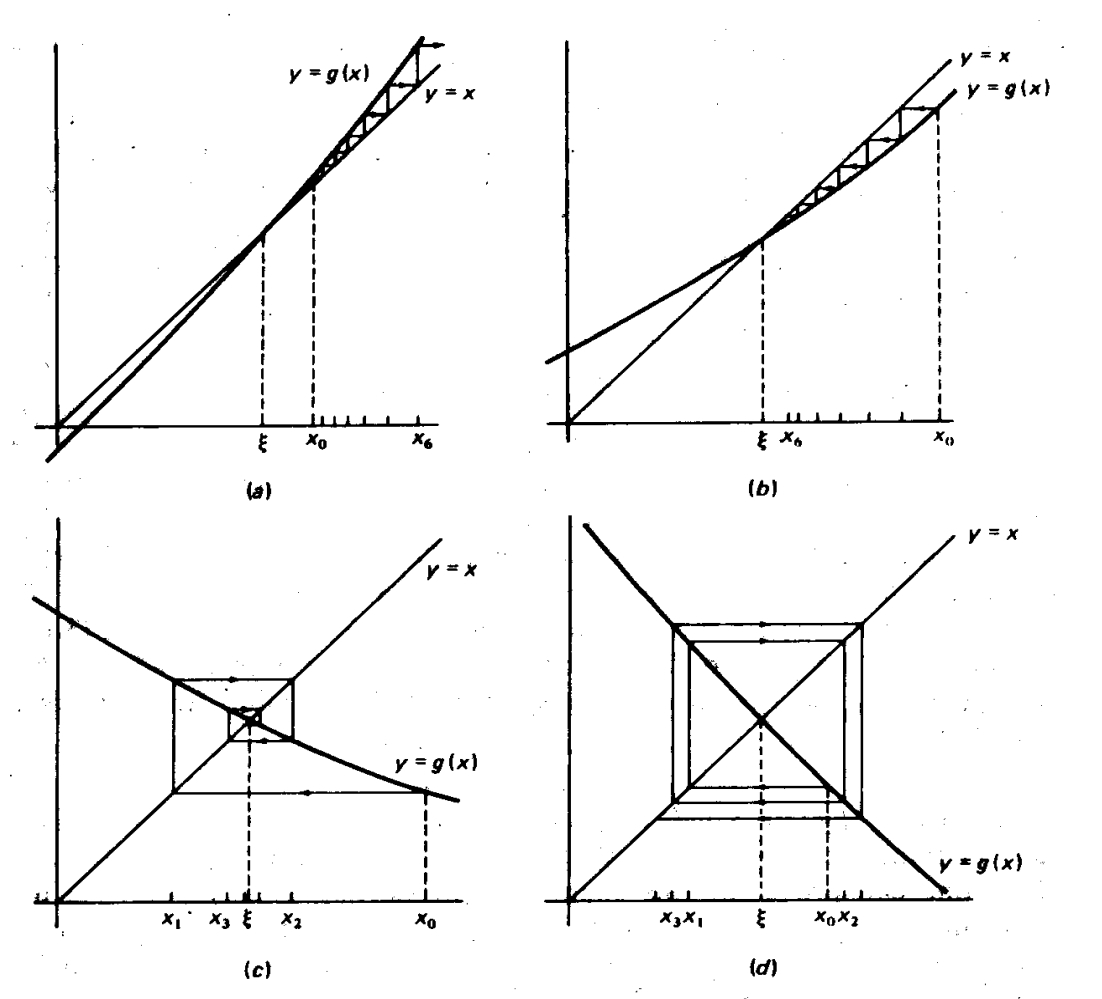
\includegraphics[width=0.6\textwidth]{figure/ne1_fixed_point_iteration_procedure.png}
    \caption{Fixed-point Iteration Procedure}
    \label{img:Fixed-point Iteration Procedure}
\end{figure}

\begin{theorem}{Convergence and Error of Fixed-Point iteration method}{convergence and Error of fixed-point iteration method}
    Assume that \\
    (1) $g,g'\in C[a,b]$;\\
    (2) $\lambda = \max_{a\leqs x\leqs b}|g'(x)|< 1$.\\
    Then \\
    (1) $x=g(x)$ has a unique solution $x^*$ in $[a,b]$.\\
    (2) For any choice of $x_0\in [a,b]$, with $x_{n+1}=g(x_n)$, $n=0,1,\dots$,
    \begin{align}
        \lim_{n\rightarrow \infty} x_n=x^*.
    \end{align}
    (3) We further have
    \begin{align}
        |x_n-x^*|\leqs \lambda^n |x_0-x^*|\leqs \frac{\lambda^n}{1-\lambda}|x_1-x_0|.
    \end{align}
\end{theorem}
\par
When using iterative methods, a natural question is when to stop the iteration?
Assume a positive number $\epsilon$ which is very small. Then, one of the following conditions may be used:\\
\textbf{Condition 1}: After each iteration check the inequality
\begin{align}
    |x_n-x_{n-k}|<\epsilon
\end{align}
for some fixed positive integer $k$. If this inequality is satisfied, 
the iteration can be stopped.\\
\textbf{Condition 2}: Another condition may be to check
\begin{align*}
    |f(x_n)|<\epsilon.
\end{align*}
This error is sometime called the residual error for the equation $f(x)=0$.


\section{Bisection Method}
Assume that $f(x)$ is continuous on a given interval $[a,b]$ 
and that is also satisfies $f(a)f(b)<0$
with $f(a)\neq 0$ and $f(b)\neq 0$.
Using the intermediate value theorem, we can see that the function $f(x)$
has at least one root in $[a,b]$.
We assume that there is only one root for the equation (\ref{eq:equations form})
in the interval $[a,b]$. The Bisection includes the following steps:\\
\textbf{Step 1}: Given an initial interval $[a_0,b_0]$, set $n=0$.\\
\textbf{Step 2}: Define $c_{n+1}=\frac{a_n+b_n}{2}$, the midpoint of the interval $[a_n,b_n]$.\\
\textbf{Step 3}:\\
If $f(a_n)f(c_{n+1})=0$, then $x^*=c_{n+1}$ is the root.\\
If $f(a_n)f(c_{n+1})<0$, then take $a_{n+1}=a_n$, $b_{n+1}=c_{n+1}$ and the root $x^*\in [a_{n+1},b_{n+1}]$.\\
If $f(a_n)f(c_{n+1})>0$, then take $a_{n+1}=c_{n+1}$, $b_{n+1}=b_n$ and the root $x^*\in [a_{n+1},b_{n+1}]$.
\\
\textbf{Step 4}: If the root is not obtained in step 3, then calculate the length of the new reduced interval $[a_{n+1},b_{n+1}]$.
If the length of the interval is less than a prescribed positive number $\epsilon$,
then take the midpoint of this interval ($x^*=\frac{a_{n+1}+b_{n+1}}{2}$) as the approximate root of the equation (\ref{eq:equations form}),
otherwise go to step 2. 
\par 
The following theorem gives the convergence and error for the bisection method.
\begin{theorem}{Convergence and Error of Bisection Method}{Convergence and Error of Bisection Method}
    Let $[a_0,b_0]=[a,b]$ be the initial interval, with $f(a)f(b)<0$.
    Define the approximate root as $x_n=\frac{b_{n-1}+a_{n-1}}{2}$.
    Then there exists a root $x^*\in [a,b]$ such that 
    \begin{align}
        |x_n-x^*|\leqs (\frac{1}{2})^n (b-a).
    \end{align} 
    Moreover, to achieve accuracy of $|x_n-x^*|\leqs \epsilon$, it suffices to take
    \begin{align}
        n\geqs \frac{\log(b-a)-\log\epsilon}{\log 2}.
    \end{align}
\end{theorem}


\section{Newton-Raphson Method}


\section{Secant Method}

\subsection{regula-falsi method}
The regula-falsi method is closely related to the bisection method. Recall the 
bisection method is to subdivide the interval $[a,b]$ in which the root lies into 
two parts, take the part of the interval which still holds the root and discard the other part of 
the interval. Although the bisection method always converges to the solution, the convergence is 
sometime very slow in the sense that if the root is very close to one of the boundary points(ie., $a$ and $b$)
of the interval. In such a situation, instead of taking the midpoint of the interval, 
we take the weighted average of $f(x)$ given by
\begin{align*}
    w=\frac{f(b)a-f(a)b}{f(b)-f(a)}.
\end{align*}
Similar to the iterative idea of Bisection Method, the regula-falsi method can defined as follows:\\
\textbf{Step 1}: Given an initial interval $[a_0,b_0]$, set $n=0$.\\
\textbf{Step 2}: Define $w_{n+1}=\frac{f(b_n)a_n-f(a_n)b_n}{f(b_n)-f(a_n)}$.\\
\textbf{Step 3}:\\
If $f(a_n)f(w_{n+1})=0$, then $x^*=w_{n+1}$ is the root.\\
If $f(a_n)f(w_{n+1})<0$, then take $a_{n+1}=a_n$, $b_{n+1}=w_{n+1}$ and the root $x^*\in [a_{n+1},b_{n+1}]$.\\
If $f(a_n)f(w_{n+1})>0$, then take $a_{n+1}=w_{n+1}$, $b_{n+1}=b_n$ and the root $x^*\in [a_{n+1},b_{n+1}]$.
\\
\textbf{Step 4}: If the root is not obtained in step 3, then calculate the length of the new reduced interval $[a_{n+1},b_{n+1}]$.
If the length of the interval is less than a prescribed positive number $\epsilon$,
then take the midpoint of this interval ($x^*=\frac{a_{n+1}+b_{n+1}}{2}$) as the approximate root of the equation (\ref{eq:equations form}),
otherwise go to step 2.


\section{Reference}
\begin{itemize}
    \item \href{https://www.math.iitb.ac.in/~baskar/book.pdf}{Introduction to Numerical Analysis ch4}
    \item \href{}{J. H. Mathews and K. D. Fink: Numerical Methods using
    MATLAB ch2, Prentice Hall of India (PHI), 4th Edition, 2005} 
\end{itemize}